\documentclass{article}

\usepackage{amsmath,amsfonts}
\usepackage[margin=3cm]{geometry}

\usepackage{multirow}

\usepackage{hyperref}
\hypersetup{
    colorlinks = true,
    linkcolor  = blue,
    urlcolor   = blue,
    citecolor  = blue
}

\usepackage{longtable}

\usepackage[numbers]{natbib}
\defcitealias{Cormen}{Cormen}

\usepackage[usenames, dvipsnames]{xcolor}
\usepackage{caption}
\usepackage{indentfirst}

\usepackage{tkz-graph}
\SetVertexNormal[Shape      = circle,
                 TextColor  = Mahogany,
                 % FillColor  = white,
                 ]
\SetUpEdge[lw         = 0.75pt,
           % color      = black,
           % labelcolor = white,
           labeltext  = ForestGreen,
           % labelstyle = {text=ForestGreen}
           ]

\usepackage{listings}
\lstdefinestyle{pseudo}
{
    keywordstyle = [1]{\normalfont\bfseries},
    keywordstyle = [2]{\normalfont\it},
    keywordstyle = [3]{\normalfont},
    morekeywords = [1]{repeat, for, to, return, if},
    morekeywords = [2]{E, n, i, j, k},
    morekeywords = [3]{let},
    morecomment = [l][\color{BrickRed}\it]{//}
}

\title{Solutions for Data Structures and Algorithms Spring 2023 — Problem Sets}
\author{By Dmitriy Okoneshnikov, B22-DSAI-04}

\begin{document}

\maketitle

\setcounter{section}{3}
\section*{Week 13. Homework 3}

\subsection{All-Pairs Shortest Paths (15 points)}
Given a directed weighted graph $G$, perform the following:
    
\begin{center}
    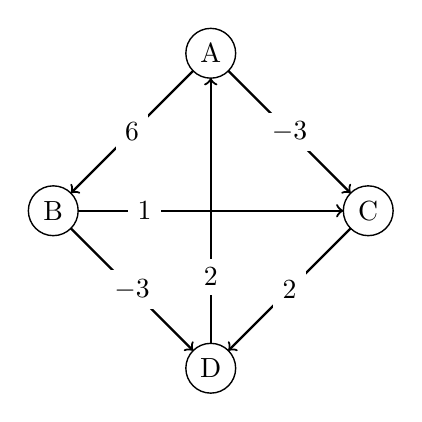
\begin{tikzpicture}
    \Vertex[x=0,y=2]{A}
    \Vertex[x=-2,y=0]{B}
    \Vertex[x=2,y=0]{C}
    \Vertex[x=0,y=-2]{D}
    \tikzset{EdgeStyle/.style = {->}}
    \Edge[label = $6$](A)(B)
    \Edge[label = $-3$](A)(C)
    \Edge[label = $1$, style={pos=.25}](B)(C)
    \Edge[label = $-3$](B)(D)
    \Edge[label = $2$](C)(D)
    \Edge[label = $2$, style={pos=.25}](D)(A)
    \end{tikzpicture}
    \captionof{figure}{Graph $G$.}
\end{center}

\begin{enumerate}
    \item Write down representation of $G$ as an adjacency matrix;

    \textbf{Answer.}

    \begin{center}
        \begin{tabular}{|c|c|c|c|c|}
            \hline
            & \textbf{A} & \textbf{B} & \textbf{C} & \textbf{D} \\
            \hline
            \textbf{A} & 0 & 6 & -3 & $\infty$ \\
            \hline
            \textbf{B} & $\infty$ & 0 & 1 & -3 \\
            \hline
            \textbf{C} & $\infty$ & $\infty$ & 0 & 2 \\
            \hline
            \textbf{D} & 2 & $\infty$ & $\infty$ & 0 \\
            \hline
        \end{tabular}
    \end{center}
    
    \item Find lengths of shortest paths between every pair of vertices in $G$ using Floyd-Warshall algorithm. Provide your solution by constructing a matrix after every iteration of the algorithm (by iteration here we mean, a choice of the intermediate vertex). The solution should have exactly 5 matrices (1 initial + 4 iterations).

    \textbf{Answer.}

    \begin{enumerate}
        \item Iteration 0:
        \begin{tabular}{|c|c|c|c|c|}
            \hline
            & \textbf{A} & \textbf{B} & \textbf{C} & \textbf{D} \\
            \hline
            \textbf{A} & 0 & 6 & -3 & $\infty$ \\
            \hline
            \textbf{B} & $\infty$ & 0 & 1 & -3 \\
            \hline
            \textbf{C} & $\infty$ & $\infty$ & 0 & 2 \\
            \hline
            \textbf{D} & 2 & $\infty$ & $\infty$ & 0 \\
            \hline
        \end{tabular}
        \item Iteration 1:
        \begin{tabular}{|c|c|c|c|c|}
            \hline
            & \textbf{A} & \textbf{B} & \textbf{C} & \textbf{D} \\
            \hline
            \textbf{A} & 0 & 6 & -3 & $\infty$ \\
            \hline
            \textbf{B} & $\infty$ & 0 & 1 & -3 \\
            \hline
            \textbf{C} & $\infty$ & $\infty$ & 0 & 2 \\
            \hline
            \textbf{D} & 2 & 8 & -1 & 0 \\
            \hline
        \end{tabular}
        \item Iteration 2:
        \begin{tabular}{|c|c|c|c|c|}
            \hline
            & \textbf{A} & \textbf{B} & \textbf{C} & \textbf{D} \\
            \hline
            \textbf{A} & 0 & 6 & -3 & 3 \\
            \hline
            \textbf{B} & $\infty$ & 0 & 1 & -3 \\
            \hline
            \textbf{C} & $\infty$ & $\infty$ & 0 & 2 \\
            \hline
            \textbf{D} & 2 & 8 & -1 & 0 \\
            \hline
        \end{tabular}
        \item Iteration 3:
        \begin{tabular}{|c|c|c|c|c|}
            \hline
            & \textbf{A} & \textbf{B} & \textbf{C} & \textbf{D} \\
            \hline
            \textbf{A} & 0 & 6 & -3 & -1 \\
            \hline
            \textbf{B} & $\infty$ & 0 & 1 & -3 \\
            \hline
            \textbf{C} & $\infty$ & $\infty$ & 0 & 2 \\
            \hline
            \textbf{D} & 2 & 8 & -1 & 0 \\
            \hline
        \end{tabular}
        \item Iteration 4:
        \begin{tabular}{|c|c|c|c|c|}
            \hline
            & \textbf{A} & \textbf{B} & \textbf{C} & \textbf{D} \\
            \hline
            \textbf{A} & 0 & 6 & -3 & -1 \\
            \hline
            \textbf{B} & -1 & 0 & -4 & -3 \\
            \hline
            \textbf{C} & 4 & 10 & 0 & 2 \\
            \hline
            \textbf{D} & 2 & 8 & -1 & 0 \\
            \hline
        \end{tabular}
    \end{enumerate}
     
\end{enumerate}

\subsection{Longest Paths (10 points)}

Consider a directed graph $P$ in which every edge has a strictly positive weight.

Graph $R$ is created from graph $P$ by reciprocating every weight (e.g. weight $5$ becomes $\frac{1}{5}$). For a given vertex $s$ in $R$ you compute all shortest paths from $s$ to every other vertex in $R$ using Dijkstra’s algorithm.

Are the following statements \texttt{TRUE} or \texttt{FALSE}? Justify your answers (providing a proof or a counterexample).

\begin{enumerate}
    \item Dijkstra’s algorithm might not be applicable to find shortest paths in $R$ (depending on original graph $P$).

    \textbf{Solution.}

    Dijkstra’s algorithm always works when the graph has no negative weights. In the problem statement it is mentioned that all weights in $P$ are strictly positive and, therefore, all weights in $R$ are also strictly positive as we get their inverse. So, the statement is false.

    \textbf{Answer.} \texttt{FALSE}
    
    \item If Dijkstra’s algorithm is applicable, the resulting shortest paths from a
vertex $s$ in $R$ correspond to the longest (i.e., with largest total weight) paths from $s$ in $P$.

    \textbf{Solution.}

    Let us take a look into one shortest path from vertex $s$ to $v$ in graph $R$. The length of this path is equal to the sum of weights of some edges $w^R_{i,j}$ that are a part of this path: $w^R_{s,a}, w^R_{a,b}, ..., w^R_{z,v}$. Due to the problem statement: $W^P{i,j}=\frac{1}{W^R{i,j}}$, Therefore, this path in graph $P$ will look like this: $\frac{1}{w^R{s,a}}, \frac{1}{w^R{a,b}}, ..., \frac{1}{w^R{z,v}}$. But $w^R{i,j}$ is the smallest number, so the inverse will be the largest. Therefore, the statement is true.

    \textbf{Answer.} \texttt{TRUE}
\end{enumerate}

\subsection{Exchanging for Profit (25 points)}

Sometimes, in the exchange market, it is possible to turn a profit by converting items or currencies in the correct order. For examples, support that one Apple share can be sold for 64 Indian rupees, one Indian rupee can buy 1.8 Japanese yen, and one yen can buy 0.009 of Apple shares. Then, by we can trade 1 Apple share for 64 Indian rupees, then trade 64 Indian rupees for 115.2 Japanese yen, which we then trade for 1.0368 Apple shares, turning a profit of 3.68\%!

In this problem, you are given $n$ different types of items or currencies $c_1, ..., c_n$ to trade with. You are also given an $n \times n$ matrix $E$ of exchange rates, such that 1 unit of $c_i$ can be exchanged for $E[i, j]$ units of $c_j$.

Perform the following:
\begin{enumerate}
    \item Give an efficient algorithm to determine whether there exists a sequence of items $c_{k_1}, c_{k_2}, ..., c_{k_m}$ such that it is possible to turn a profit simply by exchanging items:

    \[E[k_1, k_2] \cdot E[k_2, k_3] \cdot ... \cdot E[k_{m-1}, k_m] \cdot E[k_m, k_1] > 1\]

    \textbf{Answer.}

\[E[k_1, k_2] \cdot E[k_2, k_3] \cdot ... \cdot E[k_{m-1}, k_m] \cdot E[k_m, k_1] > 1\]

\[\frac{1}{E[k_1, k_2]} \cdot \frac{1}{E[k_2, k_3]} \cdot ... \cdot \frac{1}{E[k_{m-1}, k_m]} \cdot \frac{1}{E[k_m, k_1]} < 1\]

\[e^{\ln{\frac{1}{E[k_1, k_2]}} + \ln{\frac{1}{E[k_2, k_3]}} + ... + \ln{\frac{1}{E[k_{m-1}, k_m]}} + \ln{\frac{1}{E[k_m, k_1]}}} < e^0\]

\[\ln{\frac{1}{E[k_1, k_2]}} + \ln{\frac{1}{E[k_2, k_3]}} + ... + \ln{\frac{1}{E[k_{m-1}, k_m]}} + \ln{\frac{1}{E[k_m, k_1]}} < 0\]

Therefore, if we change every weight $E[i, j]$ to $\ln{\frac{1}{E[i, j]}}$ we can simplify the problem to finding a negative cycle. This can be done using Floyd-Warshall algorithm.

\begin{lstlisting}[numbers=left,language={},style=pseudo,mathescape=true,firstnumber=1]
IsNegativeCycle(E, n)
    for i:=1 to n:
        for j:=1 to n:
            if E[i,j] != INF:
                E[i,j] := log(1 / E[i,j])
    for k:=1 to n:
        for i:=1 to n:
            for j:=1 to n:
                E[i,j] := min(E[i,j], E[i,k] + E[k,j])
    for i:=1 to n:
        if E[i,i] < 0:
            return true
    return false
\end{lstlisting}

    \item Analyze the running time of your algorithm. Provide the worst case time complexity of the algorithm with justification.

    \textbf{Solution.}

    The very first update of the weights is $O(n^2)$. Then the main part of Floyd-Warshall algorithm is $O(n^3)$. The last check for negative cycles is $O(n)$. Therefore, the overall worst case time complexity of the algorithm is $O(n^3)$.

    \textbf{Answer.} $O(n^3)$
\end{enumerate}

\textit{Hint №1: reduce to a problem of finding a particular kind of cycle in a graph.}

\textit{Hint №2:} $x \cdot y = e^{\ln{x} + \ln{y}}$.

% \begin{thebibliography}{9}
% \bibitem{Cormen}
%   T. H. Cormen, C. E. Leiserson, R. L. Rivest and C. Stein.
%   \textit{Introduction to Algorithms, Fourth Edition.}
%   The MIT Press
%   2022.
% \end{thebibliography}

\end{document}
